\documentclass[10pt, a5paper]{article}
\usepackage{fontspec} 
\usepackage{verbatim} 

% DOCUMENT LAYOUT
\usepackage{geometry} 
\geometry{a5paper, textwidth=4.5in, textheight=6in, marginparsep=7pt, marginparwidth=.6in}
\setlength\parindent{0in}

% FONTS
\usepackage[usenames,dvipsnames]{color}
\usepackage{xunicode}
\usepackage{xltxtra}
\defaultfontfeatures{Mapping=tex-text}
%
\setromanfont[Scale={.8}]{TitilliumText25L}
\setmonofont[Scale=0.8]{TitilliumText25L}

% ---- CUSTOM COMMANDS
\newcommand{\amper}{{\fontspec[Scale=.95]{Linux Libertine O}\selectfont\itshape\&}}
\newcommand{\bull}{{\fontspec[Scale=.9]{Linux Libertine O}\selectfont •}}

\newcommand{\years}[1]{\marginpar{\scriptsize #1}}
\newcommand{\html}[1]{\href{#1}{\scriptsize\textsc{[html]}}}
\newcommand{\pdf}[1]{\href{#1}{\scriptsize\textsc{[pdf]}}}
\newcommand{\doi}[1]{\href{#1}{\scriptsize\textsc{[doi]}}}
\newcommand{\grey}[1]{{\bfseries\addfontfeature{Scale=.85,Color=33333399}{#1}}}
\usepackage{placeins}


% HEADINGS
\usepackage{sectsty} 
\usepackage[normalem]{ulem} 
\sectionfont{\rmfamily\bfseries\upshape\Large}
\subsectionfont{\rmfamily\bfseries\upshape\large} 
\subsubsectionfont{\rmfamily\bfseries\upshape\normalsize} 

% PDF SETUP
% ---- FILL IN HERE THE DOC TITLE AND AUTHOR
\usepackage[xetex, bookmarks, colorlinks, breaklinks, pdftitle={Giovanni Luca
Ciampaglia - portfolio},pdfauthor={Giovanni Luca Ciampaglia}]{hyperref}  
\hypersetup{linkcolor=RedViolet,citecolor=black,filecolor=black,urlcolor=RedViolet} 

\begin{document}
%
\reversemarginpar
%\raggedleft
\thispagestyle{empty}
\raggedleft
\begin{minipage}[t]{.6\linewidth}
\vspace{2cm}
{\huge\bfseries Giovanni Luca Ciampaglia}\\
\indent{\footnotesize\bfseries\addfontfeature{LetterSpace=4.6,Color=33333399}{DEVELOPER PORTFOLIO}}
\end{minipage}

%===============================================================================
% Notabilia
%===============================================================================
\newpage

\begin{minipage}[t]{.3\linewidth} 
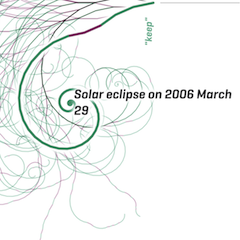
\includegraphics[width=2.5cm]{img/notabilia_kept.png}\\[.4cm]

\includegraphics[width=2.5cm]{img/notabilia_unusual.png}\\[.4cm]
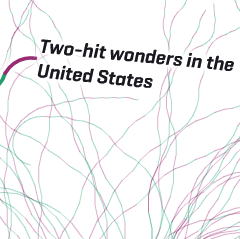
\includegraphics[width=2.5cm]{img/notabilia_two-hit.png}
\end{minipage}\hfill
\begin{minipage}[c]{.6\linewidth} 
%\vspace{1cm}
\section*{Notabilia}
\textbf{2011}\\
\grey{Flash}\\[.5cm]
\href{http://notabilia.net}{\emph Notabilia} is a visualization of the 200
longest \emph{Article for Deletion discussions} in the English Wikipedia. It's
the result of a collaboration with Moritz
Stefaner\footnote{\url{http://moritz.stefaner.eu}} (visualization) and Dario
Taraborelli\footnote{\url{http://nitens.org}} (data and analysis) and it was
launched on the occasion of the 10th anniversary of
Wikipedia.\footnote{\url{http://ten.wikipedia.org}} Article for Deletion
discussions are represented by a thread starting at the bottom center of the
screen. Each time a user recommends to keep, merge, or redirect the article a
green segment leaning towards the left is added. Each time a user recommends to
delete the article a red segment leaning towards the right is added. As the
discussion progresses, the length of the segments as well as the angle slowly
decay. 

Further analyses of deletion discussions in Wikipedia are available in a
separate paper.\footnote{\url{http://dx.doi.org/10.1109/SASOW.2010.26}}

\subsubsection*{Facts \& figures}
Notabilia is part of the
\href{http://adobemuseum.com/?/exhibit/inform/notabiliaVisualizingDeletionDiscussionsOnWikipedia}{InForm}
exhibit (2011), curated for the \href{http://adobemuseum.com/}{Adobe Museum of
Digital Media} by Thomas Goetz. 

It has also been featured in
\href{http://www.boingboing.net/2011/01/11/visualizing-the-dele.html}{BoingBoing},
\href{http://flowingdata.com/2011/01/11/visualizing-deletion-discussions-on-wikipedia/}{FlowingData},
\href{http://www.fastcodesign.com/1663011/infographic-of-the-day-the-fiery-debates-to-delete-a-wikipedia-entry}{Co.Design}
('infographic of the day'),
\href{http://www.visualizing.org/stories/visualizing-wikipedia}{Visualizing.org},
\href{http://infosthetics.com/archives/2011/01/notabilia_revealing_the_discussions_on_the_deletion_of_wikipedia_articles.html}{Information
Esthetics},
\href{http://datavisualization.ch/showcases/notabilia-–-visualizing-deletion-discussions-on-wikipedia}{DataVisualization.ch},
\href{http://www.netzpolitik.org/2011/schone-visualisierung-der-wikipedia-loschdebatten/}{NetzPolitik},
\href{http://bigthink.com/idea_feed_items/4384}{BigThink},
\href{http://www.bright.nl/bright-38}{Bright Magazine} (38/2011),
\href{http://www.page-online.de/heft/einzelheft/2011/6}{Page Magazine} (6/2011),
\href{http://twitter.com/#!/iA/status/40791557435039744}{Information
Architects}, \href{http://zoozmag.com/zooz/Home_en.html}{Zooz Magazine} and
\href{http://poptech.org/blog/truth__beauty_with_information_visualizer_moritz_stefaner}{PopTech}.
\end{minipage}
\vspace{1cm}

%===============================================================================
%Ultimatum Experiment
%===============================================================================
\newpage 
\begin{minipage}[t]{.3\linewidth}
    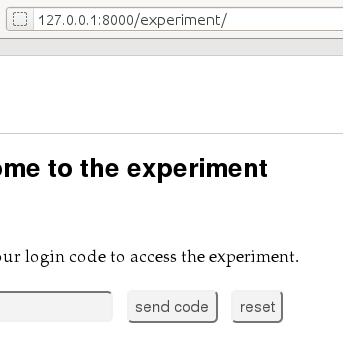
\includegraphics[width=2.5cm]{img/ultimatum_welcome.png}\\[.4cm]
    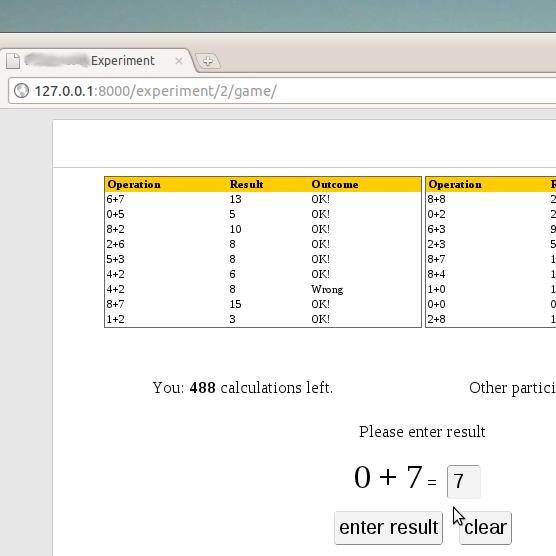
\includegraphics[width=2.5cm]{img/ultimatum_game.png}\\[.4cm]
    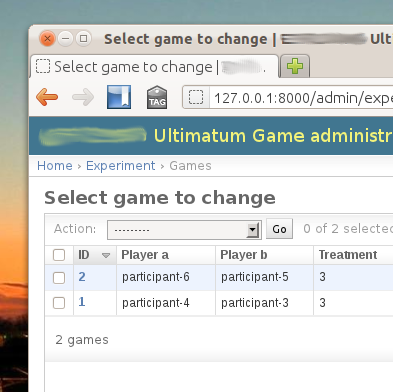
\includegraphics[width=2.5cm]{img/ultimatum_admin.png}
\end{minipage}
\hfill
\begin{minipage}[c]{.6\linewidth} 

    \section*{Ultimatum game web experiment} 

    \textbf{2011}\\ 

    \grey{Django and jQuery}\\[.5cm] 

    The ultimatum game is a two-persons experiment that is used by economists
    and sociologists to explore the nature of altruism and cooperation, usually
    in the context of monetary
    bargains.\footnote{\url{https://en.wikipedia.org/wiki/Ultimatum_game}} This
    web application implements a specific version of the ultimatum game, in
    which participants bargain over the time needed to perform a certain
    repetitive task (summing small numbers) which, upon completion, will make
    them eligible of a fixed monetary reward. The webapp was developed as part
    of a research project at the Chair of Sociology, in particular Modeling and
    Simulation of the Swiss Federal Institute of Technology of Zürich,
    Switzerland.\footnote{\url{http://www.soms.ethz.ch}} 

    \subsubsection*{Facts \& figures}
    The web app was developed using the Python web framework
    Django\footnote{\url{https://www.djangoproject.com}},
    SQLite\footnote{\url{http://sqlite.com}} and
    MySQL\footnote{\url{http://mysql.com}}. The web app takes each pair of
    players through the stages of the bargaining process with an interactive UI.
    All interactive features are implemented with the JavaScript library
    jQuery\footnote{\url{http://jquery.com}}. The webapp is optimized in terms of
    bandwidth in order to allow several pairs of participations to play the
    ultimatum game simultaneously.

\end{minipage}
\vspace{1cm}

%\hrule 
\newpage
\raggedright
\section*{Programming skills}
\textbf{Compiled languages}: Java C \bull{}
\textbf{Scripting languages:} Python Cython BASH ZSH JavaScript \bull{}
\textbf{Markup:} XHTML CSS XML JSON reStructuredText \bull{}
\textbf{Query languages:} SQL \bull{}
\textbf{Scientific packages:} R MATLAB NumPy + SciPy \bull{}
\textbf{Network analysis:} graph-tool, Gephi \bull{}
\textbf{Server administration:} Apache \bull{}
\textbf{Revision control:} Subversion Git Darcs \bull{}
\textbf{Digital typesetting:} {\fontspec[Scale=.8]{Linux Libertine O}\LaTeX\enspace\XeTeX} 

\section*{Contact}
Giovanni Luca Ciampaglia\\
36 Bertastraße\\
Zürich CH-8003\\
Switzerland\\[.2cm]
\begin{tabular}{l|l}
    T & +41 79 718 8157 \\
    T & +39 347 91 71 572 \\
    W & \href{http://www.inf.usi.ch/phd/ciampaglia}{http://www.inf.usi.ch/phd/ciampaglia}\\
    E & \href{mailto:glciampagl@gmail.com}{glciampagl@gmail.com}\\
\end{tabular}

\vfill{}
%\hrulefill
\begin{center}
{\scriptsize  \today\quad\bull{}\quad Typeset in
\href{http://nitens.org/taraborelli/latex}{XeTeX}\\\href{http://www.inf.usi.ch/phd/ciampaglia/docs/portfolio.pdf}{http://www.inf.usi.ch/phd/ciampaglia/docs/portfolio.pdf}}
\end{center}

\end{document}
